\chapter{Základní problematika virtualizace síťových funkcí}

Tato kapitola se zabývá základní analýzou a popisem problematiky spojené s oblastí virtuální síťových funkcí. V tradičních počítačových sítích je v

Routery, Firewally, IPS, IDS, Load-balancery a další.


\begin{figure}[h]
\begin{centering}
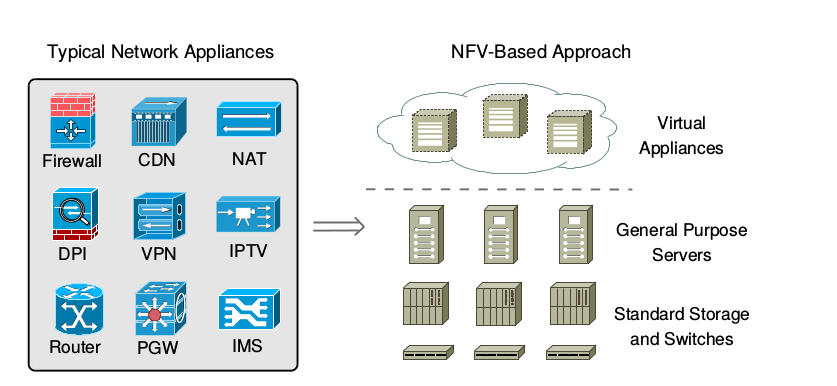
\includegraphics[scale=0.5]{images/vize_NFV}
\par\end{centering}
\caption{Koncept virtualizace síťových funkcí (NFV)\label{fig:vize_NFV}}
\end{figure}

\begin{itemize}
\item Virtualizace síťových funkcí (Network Functions Virtualization - NFV)
\item Virtuální síťové funkce (Virtual network function - VNF)
\end{itemize}

Hlavní výhody NFV:

\begin{itemize}
\item Eliminace CapEx – snížení potřeby nákupu jednoúčelových hardwarových zařízení, možnost platby pouze za využité kapacity a snížení rizik přílišného předimenzování kapacit
\item Eliminace provozních nákladů – snížení prostoru, napájení a požadavky na chlazení, zjednodušení správy a řízení síťových služeb
\item Urychlení Time-to-market –zkrácení doby pro nasazení nových síťových služeb, chopení se nových příležitosti na trhu, vyhovění potřebám zákazníka
\item Doručit agilitu a flexibilitu – možnost rychle škálovat (rozšiřovat nebo zmenšovat služby) dle měnících se požadavků od zákazníka. Podpora služeb, které mají být dodány pomocí softwaru na libovolném standartním serverovém hardwaru
\end{itemize}


\section{Souvislost NFV a SDN}\label{sub:interaction}


\section{Architektura NFV a VNF}\label{sub:interaction}

Hypervizor + hovna k tomu
Základní komponenty virtualizované platform, ve které může být NFV framework nasazen, jsou následující:


\begin{figure}[h]
\begin{centering}
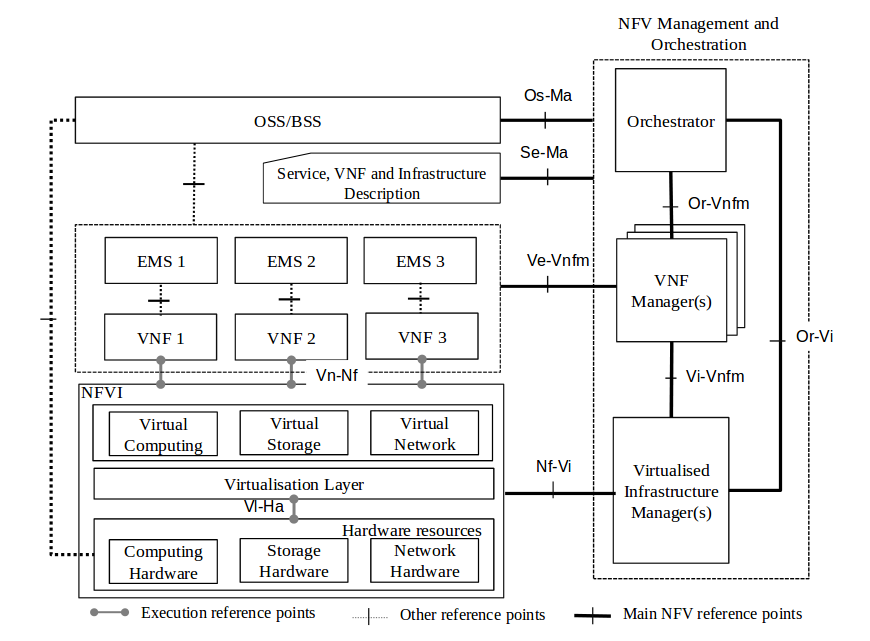
\includegraphics[scale=0.5]{images/NFV_architektura}
\par\end{centering}
\caption{NFV architektura\label{fig:NFV_architektura}}
\end{figure}


\section{Management a orchestrace NFV a VNF}\label{sub:interaction}

	\subsection{Tosca}\label{sub:interaction}

	\subsection{Netconf/Yang}\label{sub:interaction}

	\subsection{Heat engine v OpenStacku}\label{sub:interaction}

\section{}





